\chapter[CHƯƠNG MẪU-KẾT HỢP CHỮ KÝ SỐ TẬP THỂ ĐA THÀNH PHẦN VỚI CÁC MÔ HÌNH KHÁC]{KẾT HỢP CHỮ KÝ SỐ TẬP THỂ\\ ĐA THÀNH PHẦN VỚI CÁC MÔ HÌNH KHÁC} \label{chuchukykethop}  %
%\minitoc %
%\setcounter{baitap}{0}
%\thispagestyle{empty}
%\vspace*{1cm}
%%]-

%$Hash256(Hash256(blockHeaderWithoutNonce + nonce)) < target = 2^{(256-difficultyBits})$

Chương này đề xuất mô hình kết hợp giữa chữ ký số tập thể đa thành phần với chữ ký số ủy nhiệm và với chữ ký số mù. Ở mỗi loại hình kết hợp sẽ có lần lượt định nghĩa tổng quát, khả năng tấn công và đề xuất một lược đồ cụ thể để chứng minh tính đúng đắn của mô hình kết hợp.

\section{\bf Đề xuất mô hình chữ ký số tập thể đa thành phần}

\begin{figure}[ht]	
	\begin{center}		
		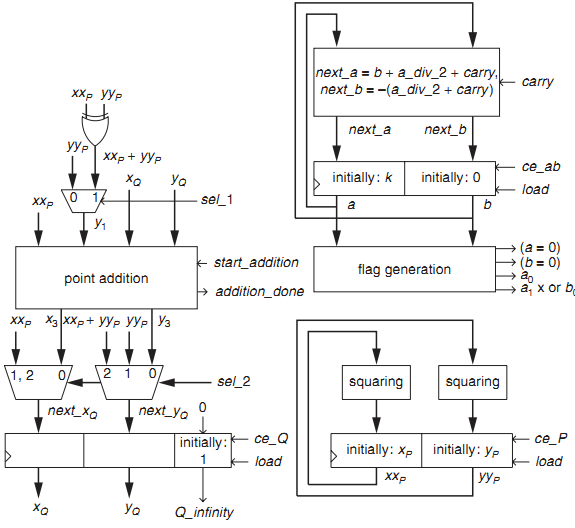
\includegraphics[scale=0.8]{nhanelliptic}
		\\		
	\end{center}	
	\caption{Phép nhân vô hướng trên đường cong elliptic}	
	\label{h.kytapthe33}
\end{figure}

Luận án đưa ra mô hình ký tập thể mới và gọi là \textit{Chữ ký số tập thể đa thành phần}. Ở đó mỗi thành viên có thể được giao cho nhiệm vụ ký một hay nhiều phần khác nhau của văn bản (các phần này không nhất thiết phải liên tục liền kề), mặt khác trong mô hình này, một thành phần của văn bản cũng có thể được một hay nhiều thành viên phụ trách và họ sẽ phải ký đồng thời vào thành phần này.


\begin{figure}[ht]	
	\begin{center}		
		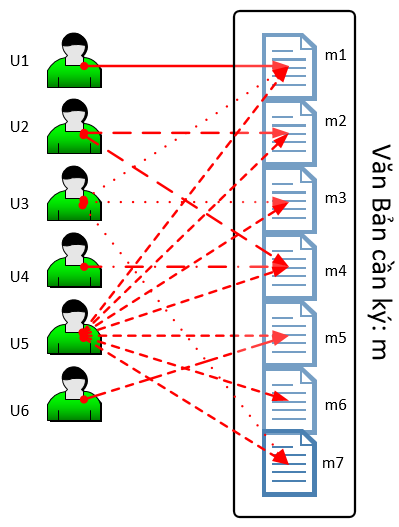
\includegraphics[scale=0.5]{kytapthe3}
		\\		
	\end{center}	
	\caption{Mô hình ký tập thể phân biệt trách nhiệm đa thành phần}	
	\label{h.kytapthe3}
\end{figure}

Hình \ref{h.kytapthe3} minh họa cho khái niệm chữ ký số tập thể đa thành phần. Ở đây có sáu người ký và văn bản được chia thành bảy phần khác nhau. Như vậy số thành viên ký trong tập thể và số thành phần văn bản được chia ra có tính độc lập tương đối với nhau. Số thành phần của văn bản có thể lớn hơn hay nhỏ hơn số thành viên của tập thể. 

Trong Hình \ref{h.kytapthe3}, có thể thấy vai trò và trách nhiệm ký của tập thể người ký như sau:
\begin{itemize}
	\item Các người ký $U1, U4, U6$ ký vào một phần của thông điệp $m$, tương ứng là các phần $m_1, m_4, m_5$.
	\item Người ký $U2$ ký và có trách nhiệm với 02 phần $m_2$ và $m_4$ của văn bản $m$.
	\item Người ký $U3$ có trách nhiệm ký với 03 phần $m_1, m_3, m_7$ của văn bản $m$.
	\item Người ký $U5$ có trách nhiệm ký tất cả các thành phần của văn bản $m$.
\end{itemize}

Mặt khác cũng trên Hình \ref{h.kytapthe3}, các thành phần của văn bản $m$ được ký bởi những người ký sau:
\begin{itemize}
	\item Thành phần $m_6$ chỉ do một người chịu trách nhiệm ký là $U5$.
	\item Các thành phần có 02 người chịu trách nhiệm ký là $m_2,m_3,m_5,m_7$.
	\item Riêng phần $m_4$ có 03 người chịu trách nhiệm ký là $U2,U4,U5$.
\end{itemize}

\begin{algorithm}%[H]
	\caption{Sinh chữ ký số ECDSA}
	INPUT: Tham số D = ($q$, FR, S, $a, b, P, n, h$), khóa bí mật $d$, thông điệp $m$. \\
	OUTPUT: Chữ ký số ($r, s$).
	\label{label1}
	\begin{algorithmic}[1]
		\STATE Chọn ngẫu nhiên $k \in [1, n-1],$ \label{tt.buoc1}
		\STATE  $R \gets kP=(x_1,y_1)$ và chuyển đổi $\bar{x_1}\gets x_1 $.
		\STATE  $r\gets\bar{x_1} \pmod n$.  
		\IF{$r=0$ or $R=\infty$} 
		\STATE Nhảy đến bước \ref{tt.buoc1}: 
		\ENDIF
		\STATE $e\gets H(m)$.
		\STATE $s \gets k^{-1}(e+dr) \pmod n$. 
		\IF{$s=0$}  
		\STATE Nhảy đến bước \ref{tt.buoc1}: 
		\ENDIF
		\STATE Trả về $(r,s)$
	\end{algorithmic}
\end{algorithm}


Đối với các tổ chức, cơ quan quản lý, văn bản $m$ có thể là công văn được phát ra, có nhiều thành phần liên quan đến chức năng của các phòng ban khác nhau trong tổ chức, có những thành phần sẽ liên quan chồng chéo giữa nhiều phòng ban và các phòng ban này phải chung nhau chịu trách nhiệm xem xét và ký duyệt.

Coi $\mathsf{NSIG}$ là tổng số các thành viên trong tập thể giam giá ký văn bản $m$, và $\mathsf{NSEC}$ là tổng số các thành phần cấu thành lên văn bản $m$. Tùy theo mối quan hệ và giá trị của $\mathsf{NSIG}$ và $\mathsf{NSEC}$ chúng ta có thể tổng hợp các mô hình ký văn bản trong Bảng \ref{bang1}. Quan sát bảng này chúng ta sẽ thấy: khi $\mathsf{NSEC}=\mathsf{NSIG}=1$ chúng ta sẽ có chữ ký số đơn. Trường hợp thứ 2 khi $\mathsf{NSIG}>1$ và $\mathsf{NSEC}=1$ chúng ta có mô hình chữ ký số tập thể không phân biệt trách nhiệm người ký. Trường hợp thứ 3 khi  $\mathsf{NSIG}>1$ và $\mathsf{NSIG}=\mathsf{NSEC}$ chúng ta có mô hình chữ ký số tập thể có phân biệt trách nhiệm người ký. Và cuối cùng là trường hợp thứ 4 khi $\mathsf{NSIG}$ và $\mathsf{NSEC}$ có giá trị bất kỳ. Qua Bảng \ref{bang1} chúng ta cũng dễ dàng nhận thấy mô hình ký tập thể đa thành phần mới được đề xuất là trường hợp tổng quát của tất cả các mô hình trước đó (ký đơn, ký tập thể không phân biệt trách nhiệm, ký tập thể có phân biệt trách nhiệm).

\begin{table}
	\centering
	\caption{Chữ ký số theo quan hệ giữa $\mathsf{NSIG}$ và $\mathsf{NSEC}$}
	\label{bang1}
	\begin{tabular}{l l p{6cm}}
		\toprule[0.125em]
		{\textsc{TT}} & {\textsc{Quan hệ}} & \textsc{{Mô hình chữ ký}}\\\toprule[0.125em]%\hline% \midrule
		1 & $\mathsf{NSIG}=1$ và $\mathsf{NSEC}=1$ & Mô hình chữ ký số đơn thông thường.\\  \midrule
		2 & $\mathsf{NSIG}>1$ và $\mathsf{NSEC}=1$ & Mô hình chữ ký số tập thể không phân biệt trách nhiệm người ký.\\\midrule
		3 & $\mathsf{NSIG}>1$ và $\mathsf{NSIG}=\mathsf{NSEC}$ & Mô hình chữ ký số tập thể phân biệt trách nhiệm người ký.\\\midrule
		4 & Với mọi $\mathsf{NSIG}$ và $\mathsf{NSEC}$  & Mô hình chữ ký số tập thể đa thành phần (có phân biệt trách nhiệm người ký).\\\bottomrule[0.125em]
	\end{tabular}
\end{table}

%\begin{center}
%	\begin{tabular}{||c c c c||} 
%		\hline
%		Col1 & Col2 & Col2 & Col3 \\ [0.5ex] 
%		\hline\hline
%		1 & 6 & 87837 & 787 \\ 
%		\hline
%		2 & 7 & 78 & 5415 \\
%		\hline
%		3 & 545 & 778 & 7507 \\
%		\hline
%		4 & 545 & 18744 & 7560 \\
%		\hline
%		5 & 88 & 788 & 6344 \\ [1ex] 
%		\hline
%	\end{tabular}
%\end{center}

\section{\bf Mô hình kết hợp chữ ký số tập thể đa thành phần và chữ ký số ủy nhiệm }

Chữ ký số ủy nhiệm là mô hình, lược đồ ký số mà ở đó một cá nhân có thể ủy quyền cho một cá nhân khác ký thay cho mình khi đi vắng. Và việc ký thay này có thể được gắn với một thuộc tính nào đó để hạn chế về điều kiện hiệu lực của việc ủy nhiệm, ví dụ như hạn chế về mặt thời gian, hạn chế về mặt nội dung, lĩnh vực ký.

\subsection{Định nghĩa chữ số tập thể ủy nhiệm đa thành phần tổng quát} \label{dnghiaTTUyNhiem}


Luận án đưa ra mô hình ký tập thể mới và gọi là \textit{Chữ ký số tập thể ủy nhiệm đa thành phần}. Ở đó mỗi thành viên có thể được giao cho nghiệm vụ ký một hay nhiều phần khác nhau của văn bản (các phần này không nhất thiết phải liên tục liền kề), mặt khác trong mô hình này, một thành phần của văn bản cũng có thể được một hay nhiều thành viên phụ trách và họ sẽ phải ký đồng thời vào thành phần này.

Giả sử có ${\mathsf{NSIG}}$ người ký $U_i$; $1\leqslant i\leqslant {\mathsf{NSIG}}$ cần ký văn bản $m \in  \{0,1\}^*$. Chia $m$ thành $\mathsf{NSEC}$ phần, sao cho có thể biểu diễn $m$ dưới dạng: \[ m= (m_1\parallel m_2\parallel m_3 \parallel \dotsm \parallel m_\mathsf{NSEC} ). \] sử dụng ký hiệu và định nghĩa mảng phân công ký $\mathfrak{V}$.

Từng thành viên $U_i$ sẽ chịu trách nhiệm ký một số phần của văn bản $m$, tính giá trị hàm băm $h_i(m_j)$; $1\leqslant j\leqslant \mathsf{NSEC}$ và gửi cho người ủy nhiệm, người này sẽ tính giá trị băm tổng hợp $H_e$. 

\begin{defi}[Chữ ký số tập thể ủy nhiệm đa thành phần - MSMS-PROXY] Giả sử văn bản $m$ được chia thành $ \mathsf{NSEC}$, có tập thể $ \mathsf{NOSIG}$ người ủy nhiệm cần ủy nhiệm quyền ký cho tập thể $ \mathsf{NPSIG}$ người ký, chữ ký tập thể ủy nhiệm đa thành phần là tập bộ 13 thành phần ($\boldsymbol{\mathsf{Setup}}$, $\boldsymbol{\mathsf{KeyGen}_{OSIG}}$, $\boldsymbol{\mathsf{KeyGenPub}_{OSIG}}$, $\boldsymbol{\mathsf{Sign}_{OSIG}}$, $\boldsymbol{\mathsf{SignPub}_{OSIG}}$, $\boldsymbol{\mathsf{Verify}_{OSIG}}$, $\boldsymbol{\mathsf{VerifyPub}_{OSIG}}$,  $\boldsymbol{\mathsf{KeyGen}_{PSIG}}$, $\boldsymbol{\mathsf{KeyGenPub}_{PSIG}}$, $\boldsymbol{\mathsf{Sign}_{PSIG}}$, $\boldsymbol{\mathsf{SignPub}_{PSIG}}$, $\boldsymbol{\mathsf{Verify}_{PSIG}}$, $\boldsymbol{\mathsf{VerifyPub}_{PSIG}}$ )  có thuật toán thực hiện trong thời gia đa thức với các giao thức sau:  \label{dn311}

\begin{enumerate}[label=(\arabic*)]
	\item Khởi tạo tham số $\mathsf{params} $ với $k$ là tham số độ an toàn, $R$ là tham số ngẫu nhiên.
	\begin{equation}
	\mathsf{params} \stackrel{R}{\longleftarrow}  \boldsymbol{\mathsf{Setup}}(1^k)
	\end{equation}
	\item Sinh khóa công khai và bí mật cho các thành viên $OSIG_i$, $1\leqslant i\leqslant \mathsf{NOSIG}$.
	\begin{equation}
	\mathsf{(PK.OSIG_i,SK.OSIG_i)} \gets \boldsymbol{\mathsf{KeyGen}_{OSIG}}(\mathsf{params},1^k, i)
	\end{equation}
	Sau khi có khóa công khai của từng thành viên, sinh khóa công khai của cả tập thể bằng thuật toán:
	\begin{equation}
	\mathsf{(PK.OSIG_{pub})} \gets \{\boldsymbol{\mathsf{KeyGenPub}_{OSIG}}(\mathsf{PK.OSIG_i})\}^{\mathsf{NOSIG}}_{i=1}
	\end{equation}	
	\item Hình thành chữ ký của tập thể người ủy nhiệm: Từng thành viên $OSIG_i$ tham gia ký văn bản theo thuật toán dưới đây:
	\begin{equation}
	\sigma.OSIG_i \gets \boldsymbol{\mathsf{Sign}_{OSIG}}^R(\mathtt{SK.OSIG_i},m)
	\end{equation}
	Người tổng hợp cần phải kiểm tra chữ ký của từng thành viên bằng thuật toán sau:
	\begin{equation}
	\{0,1\} \gets \{\boldsymbol{\mathsf{Verify}_{OSIG}}(\mathsf{PK.OSIG_{i}},m,\sigma_{i})\}^{\mathsf{NOSIG}}_{i=1}  
	\end{equation}
	Nếu tất cả đều hợp lệ (Accept) thì tiến hành tính chữ ký của cả tập thể, nếu không thì yêu cầu thực hiện lại bước này.
	\begin{equation}
	\sigma.OSIG_{pub} \gets \{\boldsymbol{\mathsf{SignPub}_{OSIG}}^R(\sigma_i)\}^{\mathsf{NOSIG}}_{i=1}
	\end{equation}
	\item Xác thực văn bản của tập thể người ủy nhiệm:
	\begin{equation}
	\{0,1\} \gets \boldsymbol{\mathsf{VerifyPub}_{OSIG}}(\mathsf{PK.OSIG_{pub}},m',\sigma.OSIG_{pub})  
	\end{equation}
	\item Sinh khóa công khai và bí mật cho các thành viên được ủy nhiệm $PSIG_j$, $1\leqslant j\leqslant \mathsf{NPSIC}$, $w$ là giá trị bảo đảm.
	\begin{equation}
	\mathsf{(PK.PSIG_j,SK.PSIG_j)} \gets \boldsymbol{\mathsf{KeyGen}_{PSIG}}(\mathsf{params},w, 1^k, j, \mathfrak{V}_j)
	\end{equation}
	Sau khi có khóa công khai của từng thành viên, sinh khóa công khai của cả tập thể bằng thuật toán:
	\begin{equation}
	\mathsf{(PK.PSIG_{pub})} \gets \{\boldsymbol{\mathsf{KeyGenPub}_{PSIG}}(\mathsf{PK.PSIG_j},\mathfrak{V}_j)\}^{\mathsf{NPSIC}}_{j=1}
	\end{equation}	
	\item Hình thành chữ ký của tập thể người ủy nhiệm: Từng thành viên $PSIG_j$ tham gia ký văn bản theo thuật toán dưới đây:
	\begin{equation}
	\sigma.PSIG_j \gets \boldsymbol{\mathsf{Sign}_{PSIG}}^R(\mathtt{SK.PSIG_j},w,m,\mathfrak{V}_j)
	\end{equation}
	Người tổng hợp cần phải kiểm tra chữ ký của từng thành viên bằng thuật toán sau:
	\begin{equation}
	\{0,1\} \gets \{\boldsymbol{\mathsf{Verify}_{PSIG}}(\mathsf{PK.PSIG_{j}},w,m,\sigma_{j},\mathfrak{V}_j)\}^{\mathsf{NPSIC}}_{j=1} 
	\end{equation}
	Nếu tất cả đều hợp lệ (Accept) thì tiến hành tính chữ ký của cả tập thể, nếu không thì yêu cầu thực hiện lại bước này.
	\begin{equation}
	\sigma.PSIG_{pub} \gets \{\boldsymbol{\mathsf{SignPub}_{PSIG}}^R(\sigma_j,\mathfrak{V})\}^{\mathsf{NPSIC}}_{j=1}
	\end{equation}
	\item Xác thực văn bản của tập thể người được ủy nhiệm:
	\begin{equation}
	\{0,1\} \gets \boldsymbol{\mathsf{VerifyPub}_{PSIG}}(\mathsf{PK.PSIG_{pub}},m',\sigma.PSIG_{pub})  
	\end{equation}
\end{enumerate}
\end{defi}


\subsection{Tấn công ACMA - Adaptive Chosen Message Attacks với mô hình MSMS-PROXY}

Đây là loại hình tấn công mạnh nhất, kẻ tấn công có thể được lựa chọn văn bản để ký phụ thuộc vào khóa công khai cũng như những chữ ký số có từ trước đó. Có thể biểu diễn việc này thông qua khả năng truy cập đến hàm Oracle, ký hiệu là $\mathsf{Sign(\cdot)}_{sk}$.

%\begin{landscape}
\begin{equation}
 \arraycolsep=1.4pt\def\arraystretch{1.7} %giãn dòng trong \begin{array}
 \resizebox{1.11\hsize}{!}{$% bóp công thức nhỏ đi
\epsilon_{\mathcal{A}}(k) \eqdefU \Pr
\left[ 
%\left( 
\begin{array}{c}
\{m_{i_m}\}^{\ell}_{i_m=1} \gets M_k;\\
\mathsf{(PK.OSIG_i,SK.OSIG_i)} \gets \boldsymbol{\mathsf{KeyGen}_{OSIG}}(\mathsf{params},1^k, i) ; \\
	\mathsf{(PK.OSIG_{pub})} \gets\{\boldsymbol{\mathsf{KeyGenPub}_{OSIG}}(\mathsf{PK.OSIG_i})\}^{\mathsf{NOSIG}}_{i=1};\\
\sigma.OSIG_i \gets \boldsymbol{\mathsf{Sign}_{OSIG}}^R(\mathtt{SK.OSIG_i},m);\\
\mathsf{(PK.PSIG_j,SK.PSIG_j)} \gets \boldsymbol{\mathsf{KeyGen}_{PSIG}}(\mathsf{params},w, 1^k, j, \mathfrak{V}_j) ; \\
\mathsf{(PK.PSIG_{pub})} \gets \{\boldsymbol{\mathsf{KeyGenPub}_{PSIG}}(\mathsf{PK.PSIG_j},\mathfrak{V}_j)\}^{\mathsf{NPSIC}}_{j=1} ;\\
\sigma.PSIG_j \gets \boldsymbol{\mathsf{Sign}_{PSIG}}^R(\mathtt{SK.PSIG_j},w,m,\mathfrak{V}_j);\\
\sigma.PSIG_{{pub}_{i_m}} \gets \{\boldsymbol{\mathsf{SignPub}_{PSIG}}^R(\sigma_j,\mathfrak{V})\}^{\mathsf{NPSIC}}_{j=1};\\
(m,\sigma.PSIG_{{pub}_{i_m}}) \gets \mathcal{A}^{\mathsf{Sign(\cdot)}_{sk}}\left( \mathsf{PK_{pub}}\right) 
\end{array} 
%\right) 
:
\begin{array}{c}
%1 \gets \left\lbrace \boldsymbol{\mathsf{Verify}}(\mathsf{PK_{i}},m,\sigma_{i},\mathfrak{V}_i)\right\rbrace_{i=1}^{\mathsf{NSIG}} ;\\
1 \gets \boldsymbol{\mathsf{VerifyPub}}(\mathsf{PK_{pub}},m,\sigma_{pub},\mathfrak{V}) \\
\wedge \quad m \notin \{m_1,\ldots,m_{\ell}\}
\end{array}
\right] 
$}
\end{equation}
\[ 
\epsilon_{\mathcal{A}}(k) \le \mathsf{negl}(k)
 \]
\begin{defi} Lược đồ MSMS-PROXY được cho là không thể giả mạo với tấn công ACMA khi với mọi thuật toán thời gian đa thức của người tấn công $\mathcal{A}$, xác suất thành công của thực nghiệm dưới đây là một hàm nhỏ không đáng kể:
	\begin{enumerate}[label=(\arabic*)]
		\item Chuỗi $\ell=\ell(k)$ văn bản $m_1,\ldots,m_{\ell}$ được chọn một cách ngẫu nhiên trong không gian $M_k$.
		\item Thực hiện các thuật toán trong lược đồ để tạo ra chữ ký $\sigma_{{pub}_{i_m}}$.
		\item Thuật toán $\mathcal{A}$ với đầu vào là $\mathsf{PK_{pub}}$ và có thể truy cập đến $\mathsf{Sign(\cdot)}_{sk}$ với một số văn bản bất kỳ và sẽ cho ra chữ ký số $(m,\sigma_{pub}) $. Không gian các văn bản truy vấn này gọi là $M$.
		\item Thực nghiệm tấn công thành công nếu $1 \gets \boldsymbol{\mathsf{VerifyPub}}(\mathsf{PK_{pub}},m,\sigma_{pub},\mathfrak{V})$ và $m\ne M$.
	\end{enumerate}	
\end{defi}
%\end{landscape}

\subsection{Đề xuất chữ ký số tập thể đa thành phần ủy nhiệm dựa trên hệ mật định danh} \label{muc.uynhiemIDBased}

%Do Rajeev Anand và Sahadeo Padhye đề xuất vào năm 2013 \cite{S10851}.

\subsubsection {Cài đặt}
Coi $G_1$ là nhóm cộng cyclic có bậc là số nguyên tố $q$ và phần tử sinh là $P$. $G_2$ là nhóm nhân cyclic có cùng bậc $q$. $e$ là một ánh xạ song tuyến tính: \[ \hat{e}: G_1 \times G_1 \to G_2 \] $H_1, H_2, H_3$ là các hàm băm được sử dụng cho mục đích bảo mật và được định nghĩa như sau:
\begin{align}
	H_1: \{0,1\}^* & \to G_1 \\
	H_2: \{0,1\}^* & \to \mathbb{Z}_q^* \\
	H_3: \{0,1\}^* \times \{0,1\}^* & \to \mathbb{Z}_q^*
\end{align}


\begin{enumerate}[label=(\arabic*)]
	\item Với tham số bảo mật $k$ chọn ngẫu nhiên $s \in \mathbb{Z}_q^*$.
	\item Tính khóa công khai của hệ thống: \[ P_{pub} = sP \in G_1 \]
	\item Công bố tham số của hệ thống là: \[ Params = (k,G_1,G_2,q,\hat{e},H_1,H_2,H_3, P,P_{pub}) \]
\end{enumerate}	

\subsubsection{Tách khóa}

Người ký ủy nhiệm có định danh là $ID$, có $\mathsf{NPSIC}$ người có thể ký ủy nhiệm $ID_{B_i}$ với $1\le i \le \mathsf{NPSIC}$.
\begin{enumerate}[label=(\arabic*)]
	\item Bất kỳ ai cũng có thể tính khóa công khai của người cần ủy nhiệm: 
	\[ Q_{ID} = H_1(ID) \in G_1 \] và những người được ủy nhiệm: \[ Q_{ID_{B_i}} = H_1(ID_{B_i}) \in G_1 \]
	\item Người quản trị hệ thống sẽ tính khóa bí mật cho người ủy nhiệm và được ủy nhiệm:
	\begin{align*}
		S_{ID} &= sQ_{ID} \\
		S_{ID_{B_i}} &= sQ_{ID_{B_i}} \quad 1\le i \le \mathsf{NPSIC}
	\end{align*}
	Người quản trị sẽ thông qua kênh bí mật gửi các khóa bí mật này cho các thành viên.
\end{enumerate}

\subsubsection{Hình thành chữ ký của người ủy nhiệm}

\begin{enumerate}[label=(\arabic*)]
	\item Với văn bản $m \in \{0,1\}^*$, người ký chọn ngẫu nhiên $x \in \mathbb{Z}_q^*$.
	\item Tính các giá trị:
	\begin{align*}
	V_s &= xP\\
	H &=H_2(m) \\
	W_s &= HS_{ID} + xP_{pub}
	\end{align*}
	\item chữ ký của người ủy nhiệm là $\sigma = (W_s,V_s)$.
\end{enumerate}	

\subsubsection{Xác thực chữ ký người ủy nhiệm}

\begin{enumerate}[label=(\arabic*)]
	\item Với văn bản $m'$ và chữ ký $\sigma = (W_s,V_s)$ nhận được, người xác thực tính: 
	 \[ H'=H_2(m') \]  \[ Q_{ID} = H_1(ID) \]
	\item Chấp nhận chữ ký khi điều kiện sau thỏa mãn:
	\begin{equation}
	\hat{e}(W_s,P) = \hat{e}(H'Q_{ID} + V_s,P_{pub})
	\end{equation}
\end{enumerate}

\subsubsection{Sinh khóa cho người được ủy nhiệm}

Trong giai đoạn này người ủy nhiệm sẽ trao đổi với người được ủy nhiệm với các quyền được ủy nhiệm. Để làm việc này người ủy nhiệm sẽ tạo ra một văn bản bảo đảm $w$, văn bản này sẽ kèm theo một số thông tin về văn bản, về những hạn chế của văn bản sẽ ủy nhiệm, thời gian hoặc định danh của những người sẽ ủy nhiệm.
\begin{enumerate}[label=(\arabic*)]
	\item \textit{Ủy nhiệm}: Người cần ủy nhiệm chọn ngẫu nhiên $t \in \mathbb{Z}_q^*$ và tính:
	\begin{align*}
	V &= tP, \\
	h &=H_2(w), \\
	W &= hS_{ID} + tP_{pub} \in G_1
	\end{align*}
	Chuyển giá trị $(W, V, w)$ với các thành viên qua kênh truyền bí mật.
	\item \textit{Kiểm tra ủy nhiệm}: mỗi thành viên $ID_{B_i}$ sẽ tính $ h =H_2(w) $ và kiểm tra điều kiện sau (nếu không thỏa mãn thì phải yêu cầu gửi lại hoặc hủy giao thức):
	\begin{equation*}
	\hat{e}(W,P) = \hat{e}(hQ_{ID} + V,P_{pub})
	\end{equation*}
	\item \textit{Sinh khóa ủy nhiệm}: mỗi thành viên $ID_{B_i}$ sẽ tính $ h =H_2(w) $ tính khóa bí mật ủy nhiệm:
	\begin{equation*}
	S_{pk_i} = W + hS_{ID_{B_i}}
	\end{equation*}
\end{enumerate}

\subsubsection{Hình thành chữ ký ủy nhiệm}
Trong pha này sẽ có một người phụ trách có nhiệm vụ tập hợp hết tất cả các chữ ký thành phần.


\begin{enumerate}[label=(\arabic*)]
	%\item Mỗi thành viên $ID_{B_i}$ sẽ chọn ngẫu nhiên số $x_i \in \mathbb{Z}_q^*$.
	\item Mỗi thành viên $ID_{B_i}$ ($1\leqslant i\leqslant \mathsf{NPSIC}$) chọn ngẫu nhiên số nguyên $x_i\in Z_q^*$ như là khóa bí mật và tính khóa công khai tương ứng theo công thức: 
	\begin{equation}
	U_{p_i}=x_iP
	\end{equation}
%	với định nghĩa phép toán:        
%	\begin{equation}
%	\mathfrak{V}_i \otimes x_i=\sum_{j=1}^\mathsf{NSEC} (\mathfrak{V}_{i}[j]\times x_{i}[j]) \pmod q 
%	\end{equation}
	Giả thiết có $\mathsf{NPSIC}$ người $ID_{B_i}$; $1\leqslant i\leqslant \mathsf{NPSIC}$ cần ký văn bản $m \in  \{0,1\}^*$. Chia văn bản $m$ thành $\mathsf{NSEC}$ phần, sao cho có thể viết $m$ theo dạng \[ m= (m_1|| m_2|| m_3 || \dots || m_\mathsf{NSEC} ) \] sử dụng ký hiệu và định nghĩa mảng phân công ký $\mathfrak{V}$ như ở Định nghĩa \ref{mangKy} (trang \pageref{mangKy}).
	
	Từng thành viên $ID_{B_i}$ sẽ chịu trách nhiệm ký một số phần của văn bản $m$, tính giá trị hàm băm $h_i(m_j)$; $1\leqslant j\leqslant \mathsf{NSEC}$ và gửi cho người ủy nhiệm, người này sẽ tính giá trị băm cho $m_j$ như sau:
	\begin{align}
	e_j &=\sum_{i=1}^{\mathsf{NSIG}} \left(\mathfrak{V}_i[j] \times h_i(m_j)\right); \quad 1\leqslant j\leqslant \mathsf{NSEC} \\
	h_3 &=H_3(e_1||e_2\cdots ||e_\mathsf{NSEC},w)
	\end{align}	
	Bằng cách tính như trên chúng ta thu được chữ ký số tập thể có phân biệt trách nhiệm, gửi giá trị $U_{p_i}$ đến $(\mathsf{NPSIC}-1)$ các thành viên còn lại.
	\item Các thành viên tính và gửi $ \sigma_{p_i} $ :
	\begin{align*}
	U_p &=\sum_{i=1}^{\mathsf{NPSIG}}U_{p_i} \\
	\sigma_{p_i} &= h_3S_{pk_i} + x_iP_{pub}
	\end{align*}
	\item Người phụ trách sau khi có các chữ ký thành phần sẽ tạo khóa công khai ủy nhiệm:
	\begin{equation}
	Q_{pk_i} = h\left(Q_{ID} + Q_{ID_{B_i}} \right)  + V
	\end{equation}
	Và sau đó kiểm tra điều kiện:
	\begin{align}
	\hat{e}(P,\sigma_{p_i}) &= \hat{e}(P_{pub},h'Q_{pk_i} + U_{p_i}) \\
	\sigma_p &=\sum_{i=1}^{\mathsf{NPSIG}}\sigma_{p_i}
	\end{align}
	sau đó chữ ký số ủy nhiệm sẽ là $(\sigma_p,V,w,U_p,\mathfrak{V})$.
\end{enumerate}

\subsubsection{Xác thực chữ ký ủy nhiệm}
Người xác thực chữ ký ủy nhiệm sau khi nhận văn bản $m'$ và chữ ký  $(\sigma_p,V,w,U_p,\mathfrak{V})$ sẽ tiến hành các bước sau:
\begin{enumerate}[label=(\arabic*)]
	\item Kiểm tra $m'$ và bảo đảm $w$ và các điều kiện liên quan.
	\item Kiểm tra sự ủy quyền của $\mathsf{NPSIG}$ người ký. Nếu không hợp lệ thì dựng lại và từ chối chữ ký.
	\item Tính các giá trị:
	\begin{align*}
	h &=H_2(w) \\
	h_3' &= H_3(m',w) \\
	Q_{pk} &= h\left[ \mathsf{NPSIG}\cdot Q_{ID} + \sum_{i=1}^{\mathsf{NPSIG}}Q_{ID_{B_i}} \right]  + \mathsf{NPSIG} \cdot V
	\end{align*}
	\item Kiểm tra điều kiện sau nếu đúng thì chấp nhận chữ ký, ngược lại là từ chối chữ ký:
	\begin{equation}
	\hat{e}(P,\sigma_p)  = \hat{e}(P_{pub},h_3'Q_{pk} + U_p)
	\end{equation}
\end{enumerate}

\begin{theorem}[Lược đồ ký tập thể ủy nhiệm đa thành phần]
	Nếu $m'=m$ thì $\hat{e}(P,\sigma_p)  = \hat{e}(P_{pub},h_3'Q_{pk} + U_p)$.
\end{theorem}

\begin{proof}
	\begin{align*}
	\hat{e}(P,\sigma_p)  &= \hat{e}(P_{pub},h_3'Q_{pk} + U_p) \\
	\hat{e}(P,\sum_{i=1}^{\mathsf{NPSIG}}\sigma_{p_i}) &= \hat{e}(P_{pub},h_3'Q_{pk} + U_p) \\
	\hat{e}(P,\sum_{i=1}^{\mathsf{NPSIG}} \left[ h_3S_{pk_i} + x_iP_{pub} \right] ) &= \hat{e}(P_{pub},h_3'Q_{pk} + U_p) \\
	\hat{e}(P,\sum_{i=1}^{\mathsf{NPSIG}}\left[ h_3\left(W + hS_{ID_{B_i}} \right)  + x_iP_{pub} \right]) &= \hat{e}(P_{pub},h_3'Q_{pk} + U_p) \\
	\hat{e}(P,\sum_{i=1}^{\mathsf{NPSIG}}\left[ h_3\left(hS_{ID} + tP_{pub} + hS_{ID_{B_i}} \right)  + x_iP_{pub} \right]) &= \hat{e}(P_{pub},h_3'Q_{pk} + U_p) \\
	\hat{e}(P,\sum_{i=1}^{\mathsf{NPSIG}}\left[ h_3\left(hsQ_{ID} + tsP + hsQ_{ID_{B_i}} \right)  + x_isP \right]) &= \hat{e}(P_{pub},h_3'Q_{pk} + U_p) \\
	\hat{e}(P_{pub},\sum_{i=1}^{\mathsf{NPSIG}}\left[ h_3\left(hQ_{ID} + tP + hQ_{ID_{B_i}} \right)  + x_iP \right]) &= \hat{e}(P_{pub},h_3'Q_{pk} + U_p) \\
	\hat{e}(P_{pub},\sum_{i=1}^{\mathsf{NPSIG}}\left[ h_3\left(hQ_{ID} + V + hQ_{ID_{B_i}} \right) \right]+ U_p) &= \hat{e}(P_{pub},h_3'Q_{pk} + U_p) \\
	\hat{e}(P_{pub},h_3\left[\sum_{i=1}^{\mathsf{NPSIG}} \left(hQ_{ID_{B_i}} \right) + \mathsf{NPSIG}\cdot hQ_{ID} + \mathsf{NPSIG}\cdot V \right] + U_p) &= \hat{e}(P_{pub},h_3'Q_{pk} + U_p) \\
	\hat{e}(P_{pub},h_3\left[h\left[ \mathsf{NPSIG}\cdot Q_{ID} + \sum_{i=1}^{\mathsf{NPSIG}} Q_{ID_{B_i}}\right]  + \mathsf{NPSIG}\cdot V \right] + U_p) &= \hat{e}(P_{pub},h_3'Q_{pk} + U_p)\\
	\hat{e}(P_{pub},h_3Q_{pk} + U_p) &= \hat{e}(P_{pub},h_3'Q_{pk} + U_p)
	\end{align*}
	Biểu thức cuối cùng đúng khi $h_3' = h_3$.	
\end{proof}

Phần phân tích hiệu năng và an toàn của lược đồ đề xuất theo mô hình an toàn đã định nghĩa rất dài và vì chương này chỉ mang tính minh họa cho việc kết hợp mô hình chữ ký số tập thể đa thành phần với mô hình chữ ký khác nên không được trình bày cụ thể ở đây.

\section{\bf Mô hình kết hợp chữ ký số tập thể đa thành phần và chữ ký số mù}

\subsection{Định nghĩa chữ ký số tập thể mù đa thành phần tổng quát} \label{dnghiaTTMu}


Luận án đưa ra mô hình ký tập thể mới và gọi là \textit{Chữ ký số tập thể mù đa thành phần}. Ở đó mỗi thành viên có thể được giao cho nghiệm vụ ký một hay nhiều phần khác nhau của văn bản (các phần này không nhất thiết phải liên tục liền kề), mặt khác trong mô hình này, một thành phần của văn bản cũng có thể được một hay nhiều thành viên phụ trách và họ sẽ phải ký đồng thời vào thành phần này.

Giả sử có $\mathsf{NSIG}$ người ký $U_i$; $1\leqslant i\leqslant \mathsf{NSIG}$ cần ký văn bản $m \in  \{0,1\}^*$. Chia $m$ thành $\mathsf{NSEC}$ phần, sao cho có thể biểu diễn $m$ dưới dạng:\[  m= (m_1\parallel m_2\parallel m_3 \parallel \dotsm \parallel m_\mathsf{NSEC} ) \] Sử dụng ký hiệu và định nghĩa mảng phân công ký $\mathfrak{V}$.

Từng thành viên $U_i$ sẽ chịu trách nhiệm ký một số phần của văn bản $m$, tính giá trị hàm băm $h_i(m_j)$; $1\leqslant j\leqslant \mathsf{NSEC}$ và gửi cho người ủy nhiệm, người này sẽ tính giá trị băm tổng hợp $H_e$ như Định nghĩa. 
 
\begin{defi}[Chữ ký số tập thể mù đa thành phần] Lược đồ chữ ký số tập thể đa thành phần là tập bộ 09 thành phần ($\boldsymbol{\mathsf{Setup}}$, $\boldsymbol{\mathsf{KeyGen}}$, $\boldsymbol{\mathsf{KeyGenPub}}$, $\boldsymbol{\mathsf{Blind}}$, $\boldsymbol{\mathsf{Sign}}$, $\boldsymbol{\mathsf{SignPub}}$, $\boldsymbol{\mathsf{UnBlid}}$, $\boldsymbol{\mathsf{Verify}}$, $\boldsymbol{\mathsf{VerifyPub}}$) có thuật toán thực hiện trong thời gia đa thức và có giao thức giữa các thành phần như sau: 
	
	\begin{enumerate}[label=(\arabic*)]
		\item Bộ khởi tạo $\boldsymbol{\mathsf{Setup}}$: đầu ra là bộ tham số $\mathsf{params} $ 
		\begin{equation}
		\mathsf{params} \stackrel{R}{\longleftarrow}  \boldsymbol{\mathsf{Setup}}(1^k)
		\end{equation}
		\item Sinh khóa công khai và bí mật cho các thành viên $U_i$, $1\leqslant i\leqslant \mathsf{NSIG}$.
		\begin{equation}
		\mathsf{(PK_i,SK_i)} \gets \boldsymbol{\mathsf{KeyGen}}(\mathsf{params},1^k, i)
		\end{equation}
		Sau khi có khóa công khai của từng thành viên, sinh khóa công khai của cả tập thể bằng thuật toán:
		\begin{equation}
		\mathsf{(PK_{pub})} \gets \{\boldsymbol{\mathsf{KeyGenPub}}(\mathsf{PK_i},\mathfrak{V}_i)\}^{\mathsf{NSIG}}_{i=1}
		\end{equation}	
		\item Người cần ký $\boldsymbol{\mathcal{U}}$ mã hóa văn bản $m$ để tạo ra bản mã $\overline{m}$ bằng thuật toán $\boldsymbol{\mathsf{Blind}}$:
		\begin{equation}
		\overline{m} \gets \{\boldsymbol{\mathsf{Blind}}(m,\mathsf{PK_i})\}^{\mathsf{NSIG}}_{i=1}
		\end{equation}
		\item Ký văn bản: Từng thành viên $U_i$ tham gia ký văn bản theo thuật toán dưới đây:
		\begin{equation}
		\overline{\sigma}_i \gets \boldsymbol{\mathsf{Sign}}^R(\mathtt{SK_i},\overline{m},\mathfrak{V}_i)
		\end{equation}
		Người tổng hợp cần phải kiểm tra chữ ký của từng thành viên bằng thuật toán sau:
		\begin{equation}
		\{0,1\} \gets \{\boldsymbol{\mathsf{Verify}}(\mathsf{PK_{i}},m,\sigma_{i},\mathfrak{V}_i)\}^{\mathsf{NSIG}}_{i=1}  
		\end{equation}
		Nếu tất cả đều hợp lệ (Accept) thì tiến hành tính chữ ký của cả tập thể, nếu không thì yêu cầu thực hiện lại bước này.
		\begin{equation}
		\overline{\sigma}_{pub} \gets \{\boldsymbol{\mathsf{SignPub}}^R(\overline{\sigma}_i)\}^{\mathsf{NSIG}}_{i=1}
		\end{equation}
		\item Người cần ký $\boldsymbol{\mathcal{U}}$ xóa mù cho chữ ký tập thể:
		\begin{equation}
		\sigma_{pub} \gets \{\boldsymbol{\mathsf{UnBlind}}^R(\overline{\sigma}_{pub},\mathsf{PK_i})\}^{\mathsf{NSIG}}_{i=1}
		\end{equation}
		\item Xác thực văn bản:
		\begin{equation}
		\{0,1\} \gets \boldsymbol{\mathsf{VerifyPub}}(\mathsf{PK_{pub}},m',\sigma_{pub},,\mathfrak{V})  
		\end{equation}
	\end{enumerate}
\end{defi}

\subsection{Tấn công ACMA - Adaptive Chosen Message Attacks với mô hình MSMS-BL}
Đây là loại hình tấn công mạnh nhất, kẻ tấn công có thể được lựa chọn văn bản để ký phụ thuộc vào khóa công khai cũng như những chữ ký số có từ trước đó. Có thể biểu diễn việc này thông qua khả năng truy cập đến hàm Oracle, ký hiệu là $\mathsf{Sign(\cdot)}_{sk}$.

%\begin{landscape}
\[ \arraycolsep=1.4pt\def\arraystretch{1.7} %giãn dòng trong \begin{array}
\epsilon_{\mathcal{A}}(k) \eqdefU \Pr
\left[ 
%\left( 
\begin{array}{c}
\{m_{i_m}\}^{\ell}_{i_m=1} \gets M_k;\\
\left\lbrace \mathsf{(PK_i,SK_i)}\gets \boldsymbol{\mathsf{Gen}}(\mathsf{params},1^k)\right\rbrace_{i=1}^{\mathsf{NSIG}} ; \\
\mathsf{PK_{pub}} \gets \left\lbrace \boldsymbol{\mathsf{GenPub}}(\mathsf{PK_i},\mathfrak{V}_i)\right\rbrace_{i=1}^{\mathsf{NSIG}} ;\\
\overline{m} \gets \{\boldsymbol{\mathsf{Blind}}(m,\mathsf{PK_i})\}^{\mathsf{NSIG}}_{i=1}; \\
\overline{\sigma}_i \gets \boldsymbol{\mathsf{Sign}}^R(\mathtt{SK_i},\overline{m},\mathfrak{V}_i) ;\\
\overline{\sigma}_{pub} \gets \{\boldsymbol{\mathsf{SignPub}}^R(\overline{\sigma}_i)\}^{\mathsf{NSIG}}_{i=1} ;\\
\sigma_{{pub}_{i_m}} \gets \{\boldsymbol{\mathsf{UnBlind}}^R(\overline{\sigma}_{pub},\mathsf{PK_i})\}^{\mathsf{NSIG}}_{i=1} ;\\
(m,\sigma_{pub}) \gets \mathcal{A}^{\mathsf{Sign(\cdot)}_{sk}}\left( \mathsf{PK_{pub}}\right) 
\end{array} 
%\right) 
:
\begin{array}{c}
%1 \gets \left\lbrace \boldsymbol{\mathsf{Verify}}(\mathsf{PK_{i}},m,\sigma_{i},\mathfrak{V}_i)\right\rbrace_{i=1}^{\mathsf{NSIG}} ;\\
1 \gets \boldsymbol{\mathsf{VerifyPub}}(\mathsf{PK_{pub}},m,\sigma_{pub},\mathfrak{V}) \\
\wedge \quad m \notin \{m_1,\ldots,m_{\ell}\}
\end{array}
\right]
\] 
\[ 
\epsilon_{\mathcal{A}}(k) \le \mathsf{negl}(k)
\] 
\begin{defi} Lược đồ MSMS được cho là không thể giả mạo với tấn công ACMA khi với mọi thuật toán thời gian đa thức của người tấn công $\mathcal{A}$, xác suất thành công của thực nghiệm dưới đây là một hàm nhỏ không đáng kể:
	\begin{enumerate}[label=(\arabic*)]
		\item Chuỗi $\ell=\ell(k)$ văn bản $m_1,\ldots,m_{\ell}$ được chọn một cách ngẫu nhiên trong không gian $M_k$.
		\item Thực hiện các thuật toán trong lược đồ để tạo ra chữ ký $\sigma_{{pub}_{i_m}}$.
		\item Thuật toán $\mathcal{A}$ với đầu vào là $\mathsf{PK_{pub}}$ và có thể truy cập đến $\mathsf{Sign(\cdot)}_{sk}$ với một số văn bản bất kỳ và sẽ cho ra chữ ký số $(m,\sigma_{pub}) $. Không gian các văn bản truy vấn này gọi là $M$.
		\item Thực nghiệm tấn công thành công nếu $1 \gets \boldsymbol{\mathsf{VerifyPub}}(\mathsf{PK_{pub}},m,\sigma_{pub},\mathfrak{V})$ và $m\ne M$.
	\end{enumerate}	
\end{defi}
%\end{landscape}

\subsection{Đề xuất chữ ký số tập thể mù đa thành phần dựa trên đường cong elliptic} \label{muc.muElliptic}

Giả sử có $\mathsf{NSIG}$ người ký $U_i$; $1\leqslant i\leqslant \mathsf{NSIG}$ cần ký văn bản $m \in  \{0,1\}^*$. Chia $m$ thành $\mathsf{NSEC}$ phần, sao cho có thể biểu diễn $m$ dưới dạng: \[ m= (m_1\parallel m_2\parallel m_3 \parallel \dotsm \parallel m_\mathsf{NSEC} ). \] Sử dụng ký hiệu và định nghĩa mảng phân công ký $\mathfrak{V}$ như ở Định nghĩa 2.1.

%Lược đồ do Popescu đề xuất \cite{S8560} dựa trên lược đồ của Harn \cite{S170}.
Có $\mathsf{NSIG}$ người ký là $U_i$, với $1 \le i \le \mathsf{NSIG}$. Quá trình sinh khóa được thực hiện như sau:
\subsubsection{Sinh khóa}
\begin{enumerate}[label=(\arabic*)]
	\item Mỗi người ký $U_i$ ($1\leqslant i\leqslant \mathsf{NSIG}$) chọn ngẫu nhiên số nguyên $d_i$ như là khóa bí mật trong khoảng $[1,q-1]$ và tính khóa công khai tương ứng như điểm:
	\begin{align*}
		Q_i &=d_iP %\\
	%	\mathfrak{V}_i \otimes d_i &=\sum_{j=1}^\mathsf{NSEC} (\mathfrak{V}_{i}[j]\times d_{i}[j]) \pmod n
	\end{align*}		
	\item Khóa công khai của cả tập thể sẽ là:
	\[ Q = \sum_{i=1}^{\mathsf{NSIG}}Q_i \]
\end{enumerate}

\subsubsection{Giao thức lược đồ ký mù tập thể}

\begin{enumerate}[label=(\arabic*)]
	\item Mỗi thành viên $U_i$ sinh cặp khóa một lần $(\overline{k}_i,\overline{R}_i)$ bằng cách chọn ngẫu nhiên $k_i \in [1,q-1]$ và tính: \[ \overline{R}_i = (\mathfrak{V}_i \otimes k_i)P = (x_{\overline{k}_i},y_{\overline{k}_i}) \]
	Tính $\overline{r}_i = c(x_{\overline{k}_i})$ và gửi $\overline{r}_i$ tới người cần ký.
	\item Người cần ký sẽ chọn hệ số mù $a,b \in [1,q-1]$ và tính điểm $R$ trên đường cong elliptic $E$, tính: \[ \overline{R} = \sum_{i=1}^{\mathsf{NSIG}} \overline{R_i} = (x_{\overline{R}},y_{\overline{R}}) \] 
	gọi $c()$ là hàm chuyển đổi từ điểm sang giá trị tọa độ theo trục $x$ từ đó tính $\overline{r} =  c(x_{\overline{R}})$ và tính:
	\[ R = a\overline{R} + bQ  = (x_R,y_R)\]
	Tiếp theo tính giá trị $r = c(x_R)$ và:
	\begin{equation}
	\overline{m} = (H(m) + r + b)a^{-1}  - \overline{r}
	\end{equation}
	Và gửi các giá trị $\overline{m},\overline{r}$ tới các thành viên $U_i$.
	\item Các thành viên $U_i$ với $1 \le i \le \mathsf{NSIG}$ ký văn bản mù bằng cách tính:
	\begin{equation}
	\overline{s}_i = d_i(\overline{m} + \overline{r}) + (\mathfrak{V}_i \otimes k_i) \pmod q \label{pt.si}
	\end{equation}
	Gửi giá trị này tới người cần ký.
	\item Người cần ký tính:
	\begin{equation}
	R_{e_i} = (x_{e_i}, y_{e_i}) = \overline{s}_iP - (\overline{m} + \overline{r})Q_i 
	\end{equation}
	Và kiểm tra $r_i = c(x_{e_i}) \pmod q$ và tính: 
	\begin{align}
		\overline{s} &= \sum_{i=1}^{\mathsf{NSIG}} \overline{s}_i \label{pt.ssa} \\ 
		s &= \overline{s}a \pmod q \label{pt.sa}
	\end{align}
	Chữ ký mù tập thể của văn bản $m$ sẽ là $(r,s,\mathfrak{V})$.
\end{enumerate}

\subsubsection{Xác thực chữ ký mù tập thể}

Người xác thực nhận được văn bản $m'$ và chữ ký $(r,s)$. Tính giá trị:
\begin{equation}
(x_e,y_e) = sP -(H(m) + r)Q 
\end{equation}
Kiểm tra điều kiện $r = c(x_e) \pmod q$ nếu thỏa mãn thì chữ ký hợp lệ.
\[ sP -(H(m) + r)Q = R\]

\begin{theorem}[Lược đồ ký tập thể mù đa thành phần]
	Nếu $m'=m$ thì $sP -(H(m) + r)Q = R$.
\end{theorem}
\begin{proof}
	\begin{align*}
		R &=  a\overline{R} + bQ = a\sum_{i=1}^{\mathsf{NSIG}}\overline{R}_i + bQ \\
		&= a\sum_{i=1}^{\mathsf{NSIG}}\overline{R}_i + \left((\overline{m} + \overline{r})a -H(m) -r \right) Q \\
		&= a\left( \sum_{i=1}^{\mathsf{NSIG}} \left( (\mathfrak{V}_i \otimes k_i) + d_i(\overline{m} + \overline{r})\right) \right)P
		- \left(H(m) + r \right)Q \\
		&= 	a\sum_{i=1}^{\mathsf{NSIG}}\overline{s}_iP - \left(H(m) + r \right)Q \\
		&= 	a\overline{s}P - \left(H(m) + r \right)Q \\
		&= 	sP - \left(H(m) + r \right)Q 
	\end{align*}	
\end{proof}

\subsubsection {Phân tích độ an toàn của lược đồ chữ ký mới và thảo luận}


Phương pháp tấn công có thể là xây dựng thuật toán để giả mạo chữ ký $(r,s)$. Giá trị $r$ có thể dễ dàng tính được thông qua các khóa công khai của các thành viên, tuy nhiên để có được thành phần $s$, người tấn công bắt buộc phải tìm được cả $\overline{s}$ và $a$ theo (\ref{pt.sa}). Và đây là bài toán phân tích ra thừa số, là một bài toán khó. Hoặc xây người tấn công có thể xây dựng thuật toán mới để tính $\overline{s}$. Theo các công thức (\ref{pt.ssa}) và (\ref{pt.si}) để tính được $\overline{s}$ thì cần phải tìm được các giá trị $\overline{m}$, $d_i,k_i$ và để tính được các giá trị này người tấn công buộc phải giải bài toán (\ref{pt.si}) phân tích ra thừa số.

\section{\bf Kết luận chương \ref{chuchukykethop} }

Chương \ref{chuchukykethop}, Luận án cũng trình bày về đề xuất mô hình ký kết hợp giữa chữ ký tập thể đa thành phần với chữ ký mù. Cũng tương tự như ở mô hình kết hợp với chữ ký số ủy nhiệm NCS cũng mô tả dạng tấn công ACMA đối với mô hình kết hợp với chữ ký số mù. Để chứng minh cho tính đúng đắn của mô hình kết hợp giữa chữ ký số tập thể đa thành phần và chữ ký số mù, NCS đã đề xuất một lược đồ cụ thể ký tập thể đa thành phần với chữ ký mù. Các kết quả nghiên cứu trong chương này đã được công bố trong các công trình [CT6], [CT7], [CT8].%, ngoài việc phân tích đánh giá hiệu năng và độ an toàn Luận án còn nêu một số vấn đề thảo luận về mô hình ký mới này.